\section{Class diagram} \label{sec:classdiagram}
The qualified classes from \cref{sec:Classes} are ordered in relation to each other in a class diagram, the purpose of which is ``to describe structural relations between classes and objects'' \citep[p.~71]{Rod-Aalborg}.

The class diagram in \cref{fig:ClassDiagram} shows the structure between the classes in the problem domain.
The two main problems modeled in this diagram are the handbook and the suppliers.
Both of these deal with archiving and managing the documents a company needs to get their certifications.

\begin{figure}[H]
	\centering
	\begin{tikzpicture}[align=center, scale=1.0, transform shape]
	%De enkelte noder i diagrammet
	\node(start)[process]{Company};
	\node(supp)[process, below=1cm of start, xshift=-1cm]{Supplier};
	\node(hand)[process, below=1cm of start, xshift=1cm]{Handbook};
	\node(app)[process, left=0.8cm of supp]{Approval};
	\node(suppapp)[process, below=1cm of supp, xshift=-0.5cm]{Supplier Approval};
	\node(handapp)[process, below=1cm of app, xshift=-1.8cm]{Handbook Approval};
	\node(doc)[process, below=1cm of hand, xshift=0.5cm]{Document};
	\node(ver)[process, below=1cm of suppapp]{Version};
	\node(read)[process, right=2cm of ver]{Read Status};
	\node(user)[process, right=1.5cm of read]{User};
	\node(dep)[process, right=1.5cm of doc]{Department};
	\node(role)[process, below=0.6cm of user]{Role};
	\node(admin)[process, below=1cm of role, xshift=0.5cm]{Administrator};
	\node(write)[process, left=1cm of admin]{Writer};
	\node(reader)[process, left=1cm of write]{Reader};

	%linjer til company
	\draw[{open diamond}-](start.south)-- node[anchor=east]{1} (0.0,-1.0);
	\draw[black](supp.north)  |-node[below=0.2cm, left]{0..*} (0.0,-1.0) ;
	\draw[black](hand.north) |-  node[below=0.2cm, right]{1}(0.0,-1.0);
	%linje supp & suppapp
	\draw[{open diamond}-](supp.south) node[above=-0.2cm, left]{1}--(-1.0,-3.18) node[below=-0.2cm, right]{1};
	%linje til handbook & doc
	\draw[{open diamond}-](hand.south) node[above=-0.2cm, left]{1}--(1.0,-3.18) node[below=-0.2cm, right]{0..*};
	%approval linjer
	\draw[arrow](-3.55,-2.7)--(app.south);
	\draw[black](handapp.north)|-(-3.55,-2.7);
	\draw[black](suppapp.north)|-(-3.55,-2.7);
	%linjer til version &suppapp /doc
	\draw[{open diamond}-](-2.0,-3.95)node[above=-0.2cm, right]{1}--(-2.0,-4.95)node[below=-0.2cm, left]{1..*};
	\draw[{open diamond}-](1.0,-3.95)node[above=-0.2cm, left]{1}--(1.0,-4.5);
	\draw[black](1.0,-4.5)-|(ver.north)node[below=-0.2cm, right]{0..*};
	%linje user & department
	\draw[{open diamond}-](5.59,-3.95)node[above=-0.2cm, left]{1}--(user.north)node[below=-0.2cm, right]{1..*};
	%linje hanbook & user
	\draw[black](hand.east) -| (6.7,-5.0);
	\draw[black](user.east) -| (6.7,-5.0);
	%Handbook approval og user
	\draw[black](handapp.west)node[below=0.6cm, right]{1..*} -| (-7.3,-5.0);
	\draw[black] (-7.3,-5.0) |- (-6,-9.0);
	\draw[black] (user.south east)node[below=0.2cm, right]{0..*} -| (7.7,-7.0);
	\draw[black] (-6,-9.0) -| (7.7,-7.0);
	%rollemønstret
	\draw[arrow](role.north)--(user.south);
	\draw[arrow](5.63,-7.7)--(role.south);
	\draw[black](admin)|-(5.63,-7.7);
	\draw[black](reader)|-(5.63,-7.7);
	\draw[black](write)|-(5.63,-7.7);
	%Andre linjer
	\draw[black](ver.east) node[above=0.2cm,right]{1} --(read.west) node[below=0.2cm,left]{0..*};
	\draw[black](doc.east) node[above=0.2cm,right]{1} --(dep.west) node[below=0.2cm,left]{0..*};
	\draw[black](read.east) node[above=0.2cm,right]{0..*} --(user.west) node[below=0.2cm,left]{1};
	\draw[black](6.85,-8.14)node[above=0.2cm,right]{1..*}|-(start);
	\draw[black](handapp.south) node[above=-0.2, left]{0-1}|- (ver.west) node[below=0.2cm,left]{1};
	\end{tikzpicture}
	\caption{Class diagram of the problem domain}\label{fig:ClassDiagram}
\end{figure}

\subsection{Supplier}
The less complex subproblem is that of managing the suppliers.
There can be any number of suppliers, and these suppliers in turn aggregate approvals.
These approvals are meant to signify a specific period of time that the supplier is approved.
Each Approval then aggregates at least one Version, which each encapsulates one of the files needed to document the validity of approving the supplier.
This is a hierarchy pattern where both Company and Version is also included in the hierarchy structure for the handbook.
These two classes connect the two subproblems.

\subsection{Handbook}\label{sec:classdiagramhandbook}
Where a company can have multiple or no suppliers there can only be one Handbook.
The Handbook is a part of the Company which acts as a handle to access both suppliers and the handbook. This is a composition relation.

A handbook is an aggregation of Document, as there are multiple documents in each handbook, and Document is again an aggregation of versions, which keeps track of the multiple versions each document has and dates of the period one was valid in the handbook.

The relation between Document and Version is an item-descriptor pattern.
The Document class is the descriptor and contains all the important information about the document, including a pointer to the current valid version of said document.
Version is an item as it encapsulates the actual file with the current version of Document.
This is modeled so because of the need to keep track of earlier versions as well.

Version has two relational patterns, one to the Approval class and one to the Read Status class.
Both classes exist because of the need to keep the information about when an event happened and which users were involved.
Who approved this version and when did that happen?
Who has read this version of the document?
As well as the reverse: Who has not?
Keeping track of the when is important because a new version should not replace the former one before it has been approved.
Furthermore, for certification purposes it is relevant to know who has read the current version at any given time.

Document has a relation to Department.
This is because the handbook can become quite extensive, but most users only regularly need to access a couple of documents.
Therefore users should be shown specific documents relevant to them first and Department connects a group of documents to a group of users.
These departments are managed by the administrators of the system.

\subsection{User}\label{sec:user}
There are three different types of users in the system, which has been modeled by using a role pattern. This gives the system a more dynamic way to handle different contexts.

The reader can read everything and verify that they have read a version of a document but nothing else.
Every single user in the system has this level of access and it is therefore unnecessary to include as a seperate class.
However, it is an important group and therefore, for the sake of clarity, it was included as a role in the model nevertheless.

The writer has the additional permission of submitting new versions of documents for approval. They can also assign other users to approve these documents, where anyone no matter the role can be assigned.

The administrator has all access to the system.
This includes making completely new documents, managing who gets notifications for which documents through the Department class, adding and removing users and accessing the archive.
There needs to be at least one administrator per Company.

The pattern functions like a hierarchy where the reader is at the bottom level, the writer at the middle level and the administrator at the top level. This means each role have the same core attributes, but their privileges are greater for each level, increasing from bottom to top.
This relation is pictured in \cref{fig:RoleIllustration}.

\begin{figure}[H]
	\centering
	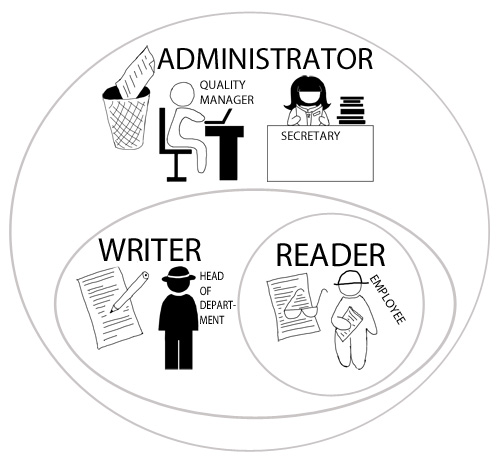
\includegraphics[width=0.75\textwidth]{billeder/RP-Roller2.jpg}
	\caption{\textit{Illustration of the different roles
	}\label{fig:RoleIllustration}}
\end{figure}

It is expected that there will be between two and three administrators in the system, and any number of writers and users.
The company's quality manager should be an administrator and will be the person most accustomed to the system.
Additionally the secretaries will need the same level of access to do their job, but they likely won't spend as much time working with the system.
The CEO of the company could also be an administrator but depending on their involvement they could also be a writer or even reader.
The writer role would typically be assigned to people like the department heads as they are the experts on how their own departments work.
Every single employee should be a user and will by default have a reader role.

\subsection{Approval} \label{Approval}
The biggest similarities between the handbook and supplier-approval subproblems are the need for archiving documents and the need for approving certain things with different intervals.

The difference between them is first and foremost that while the company needs both, they do not need each other.
The approval of the suppliers is not included in the handbook and has no relevance for the majority of the users of the handbook, and what the handbook says is irrelevant to whether a supplier is approved or not.

\begin{figure}[H]
	\centering
	\begin{tikzpicture}[align=center, scale=1.0, transform shape]
	%De venstre noder
	\node(supp)[process]{Supplier};
	\node(title)[simple, above=0.5cm of supp]{Supplier-Approval\\Subproblem};
	\node(app)[process, below=1cm of supp]{Approval};
	\node(doc)[process, below=1cm of app]{Document};
	%De højre noder
	\node(title2)[simple, right=2cm of title]{Handbook\\ Subproblem};
	\node(hand)[process, below=0.5cm of title2]{Handbook};
	\node(doc2)[process, below=1cm of hand]{Document};
	\node(ver)[process, below=1cm of doc2]{Version};
	\node(App)[process, right=1cm of ver]{Approval};

	%linjer
	\draw[black, ultra thick](title.south west)--(title.south east);
	\draw[black, ultra thick](title2.south west)--(title2.south east);
	\draw[{open diamond}-](supp)--(app);
	\draw[{open diamond}-](app)--(doc);
	\draw[{open diamond}-](hand)--(doc2);
	\draw[{open diamond}-](doc2)--(ver);
	\draw[black](ver)--(App);
	\end{tikzpicture}
	\caption{Class diagram of the problem domain
		}\label{fig:SupProblemClassDiagram}
\end{figure}

Early versions of the class diagram modeled the problems like seen in \cref{fig:PseudoClassDiagram}.
Here the classes Approval and Document are present in both diagrams, suggesting that their functionalities are too similar to have separate classes.
However, in the handbook, Document is merely a container for Versions, which include the actual files and those files are needed in supplier-approval.
Therefore, the two Document classes cannot be merged, but the Document class in supplier-approval can be entirely replaced by the Version class in handbook.

The two Approval classes are more complicated as the approval process varies:

\begin{itemize}
  \item In the handbook system a version of a document needs to be approved and the author can specify which people should do so.
  \item In the supplier-approval system a supplier needs to be approved which only demands an approval from one administrator.
\end{itemize}

However the administrator needs to submit some kind of documentation, that justifies the approval of the supplier.
Both systems need the approval for the changes to take effect.

The current version of the class diagram in \cref{fig:ClassDiagram} does this by including a generalization. The approvals' shared functionality is included in the abstract class Approval and the more specific functionalities in the subclasses HandbookApproval and SupplierApproval.
Just like in the early version of the class diagram SupplierApproval is aggregated by Version and Version contains a reference to HandbookApproval.
In the case where a Version object belongs to a SupplierApproval object the relation to HandbookApproval is set to a null reference.

The handbook part of the problem is the clients main concern and therefore the focus of this project.
In order to understand the problem in its entirety both subproblems are analyzed in this section, but from here on  only the Handbook problem will be analyzed and eventually designed, implemented and tested.
Therefore, the final class diagram looks like in \cref{fig:ClassDiagramNoSupplier}.

\begin{figure}[H]
	\centering
	\begin{tikzpicture}[align=center, scale=1.0, transform shape]
	%De enkelte noder i diagrammet
	\node(hand)[process]{Handbook};
	\node(doc)[process, below=1cm of hand]{Document};
	\node(app)[process, left=2cm of hand]{Approval};
	\node(handapp)[process, below=1cm of app]{Handbook Approval};
	\node(ver)[process, below=1cm of handapp]{Version};
	\node(read)[process, below=1cm of doc]{Read Status};
	\node(dep)[process, right=1.7cm of doc]{Department};
	\node(user)[process, below=1cm of dep]{User};
	\node(role)[process, below=0.6cm of user]{Role};
	\node(write)[process, below=1cm of role]{Writer};
	\node(reader)[process, left=1cm of write]{Reader};
	\node(admin)[process, right=1cm of write]{Administrator};

	%Linjer
	%Ver to doc
	\draw[{open diamond}-](doc.south) node[below=0.2cm, right]{1} |- (-2.0,-2.7);
	\draw[black] (-3.75,-3.2) node[above=0.25cm, right]{0..*} |- (-2.0,-2.7);
	%approval linjer
	\draw[arrow](handapp.north)--(app.south);
	\draw[black](handapp.south)node[above=-0.2cm, left]{0-1}--(ver.north) node[below=-0.2cm, left]{1};
	%rollemønster
	\draw[arrow](role.north)--(user.south);
	\draw[arrow](write.north)--(role.south);
	\draw[black](reader.north)|-(4.0,-6.0);
	\draw[black](admin.north)|-(4.0,-6.0);
	%Handbook & user
	\draw[black](hand.east)-|(6.0,-3.0);
	\draw[black](user.east)-|(6.0,-3.0);
	%Handbook approvals og user
	\draw[black](handapp.west)node[below=0.6cm, right]{1..*} -| (-6.0,-7.4);
	\draw[black] (user.south east)node[below=0.2cm, right]{0..*} -| (8.5,-7.4);
	\draw[black] (-6.0,-7.4) |- (8.5,-7.4);
	%nemme linjer
	\draw[black](doc.east) node[below=0.2cm, right]{1}--(dep.west) node[above=0.2cm, left]{0..*};
	\draw[black](ver.east) node[below=0.2cm, right]{1}--(read.west) node[above=0.2cm, left]{0..*};
	\draw[black](read.east) node[below=0.2cm, right]{0..*}--(user.west) node[above=0.2cm, left]{1};
	\draw[{open diamond}-](hand.south) node[above=-0.2cm, left]{1}--(doc.north)node[below=-0.2cm, right]{0..*};
	\draw[{open diamond}-](dep.south)node[above=-0.2cm, left]{1}--(user.north)node[below=-0.2cm, right]{1..*};
	\end{tikzpicture}
	\caption{Final class diagram of the problem domain excluding the supplier
	}\label{fig:ClassDiagramNoSupplier}
\end{figure}

In this diagram the Supplier and the SupplierApproval are not included.
As the company class mainly existed to support the administrators access to the supplier system that class and its relation to the admin role have also been excluded.
The abstract Approval class still exists to make it possible to implement the supplier system at a later time.
